% Generated by code/draw_circuits.py.
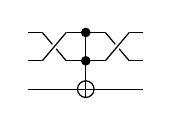
\begin{tikzpicture}[x=1cm,y=1cm,baseline={([yshift=-0.25em]mid)},line width=.45pt]
\coordinate (mid) at (0,-0.360);
\draw (0,0.000)--(1.460,0.000);
\draw (0,-0.360)--(1.460,-0.360);
\draw (0,-0.720)--(1.460,-0.720);
\draw[white,line width=2pt] (0.178,0.000)--(0.482,0.000) (0.178,-0.360)--(0.482,-0.360);
\draw (0.178,0.000)--(0.482,-0.360);
\draw[white,line width=2pt] (0.178,-0.360)--(0.482,0.000);
\draw (0.178,-0.360)--(0.482,0.000);
\draw (0.730,0.000)--(0.730,-0.720);
\filldraw[fill=black] (0.730,0.000) circle[radius=1.5pt];
\filldraw[fill=black] (0.730,-0.360) circle[radius=1.5pt];
\draw[fill=white] (0.730,-0.720) circle[radius=3pt];
\draw (0.625,-0.720)--(0.835,-0.720) (0.730,-0.825)--(0.730,-0.615);
\draw[white,line width=2pt] (0.978,0.000)--(1.282,0.000) (0.978,-0.360)--(1.282,-0.360);
\draw (0.978,0.000)--(1.282,-0.360);
\draw[white,line width=2pt] (0.978,-0.360)--(1.282,0.000);
\draw (0.978,-0.360)--(1.282,0.000);
\end{tikzpicture}
